\documentclass[11pt]{report}
\usepackage{adjustbox}
\usepackage{xcolor}

\topmargin=0.0in %length of margin at the top of the page (1 inch added by default)
\oddsidemargin=0.0in %length of margin on sides for odd pages
\evensidemargin=0in %length of margin on sides for even pages
\textwidth=6.5in %How wide you want your text to be
\marginparwidth=0.5in
\headheight=0pt %1in margins at top and bottom (1 inch is added to this value by default)
\headsep=0pt %Increase to increase white space in between headers and the top of the page
\textheight=9.0in




\begin{document}

%%%%%%%%%%%%%%%%%%%%%%%%%%%%%%%%%%%%%%%%%%%%%%%%%%%%%%%%%%%%%%%%%%%%%%%%%%%%
\begin{titlepage}
\begin{center}
\textsc{\LARGE University of Pittsburgh}\\[1.5cm]
{ \huge \bfseries STEPUP Observing Guidelines\\[0.4cm] } 


\begin{figure}[!h]
\begin{center}
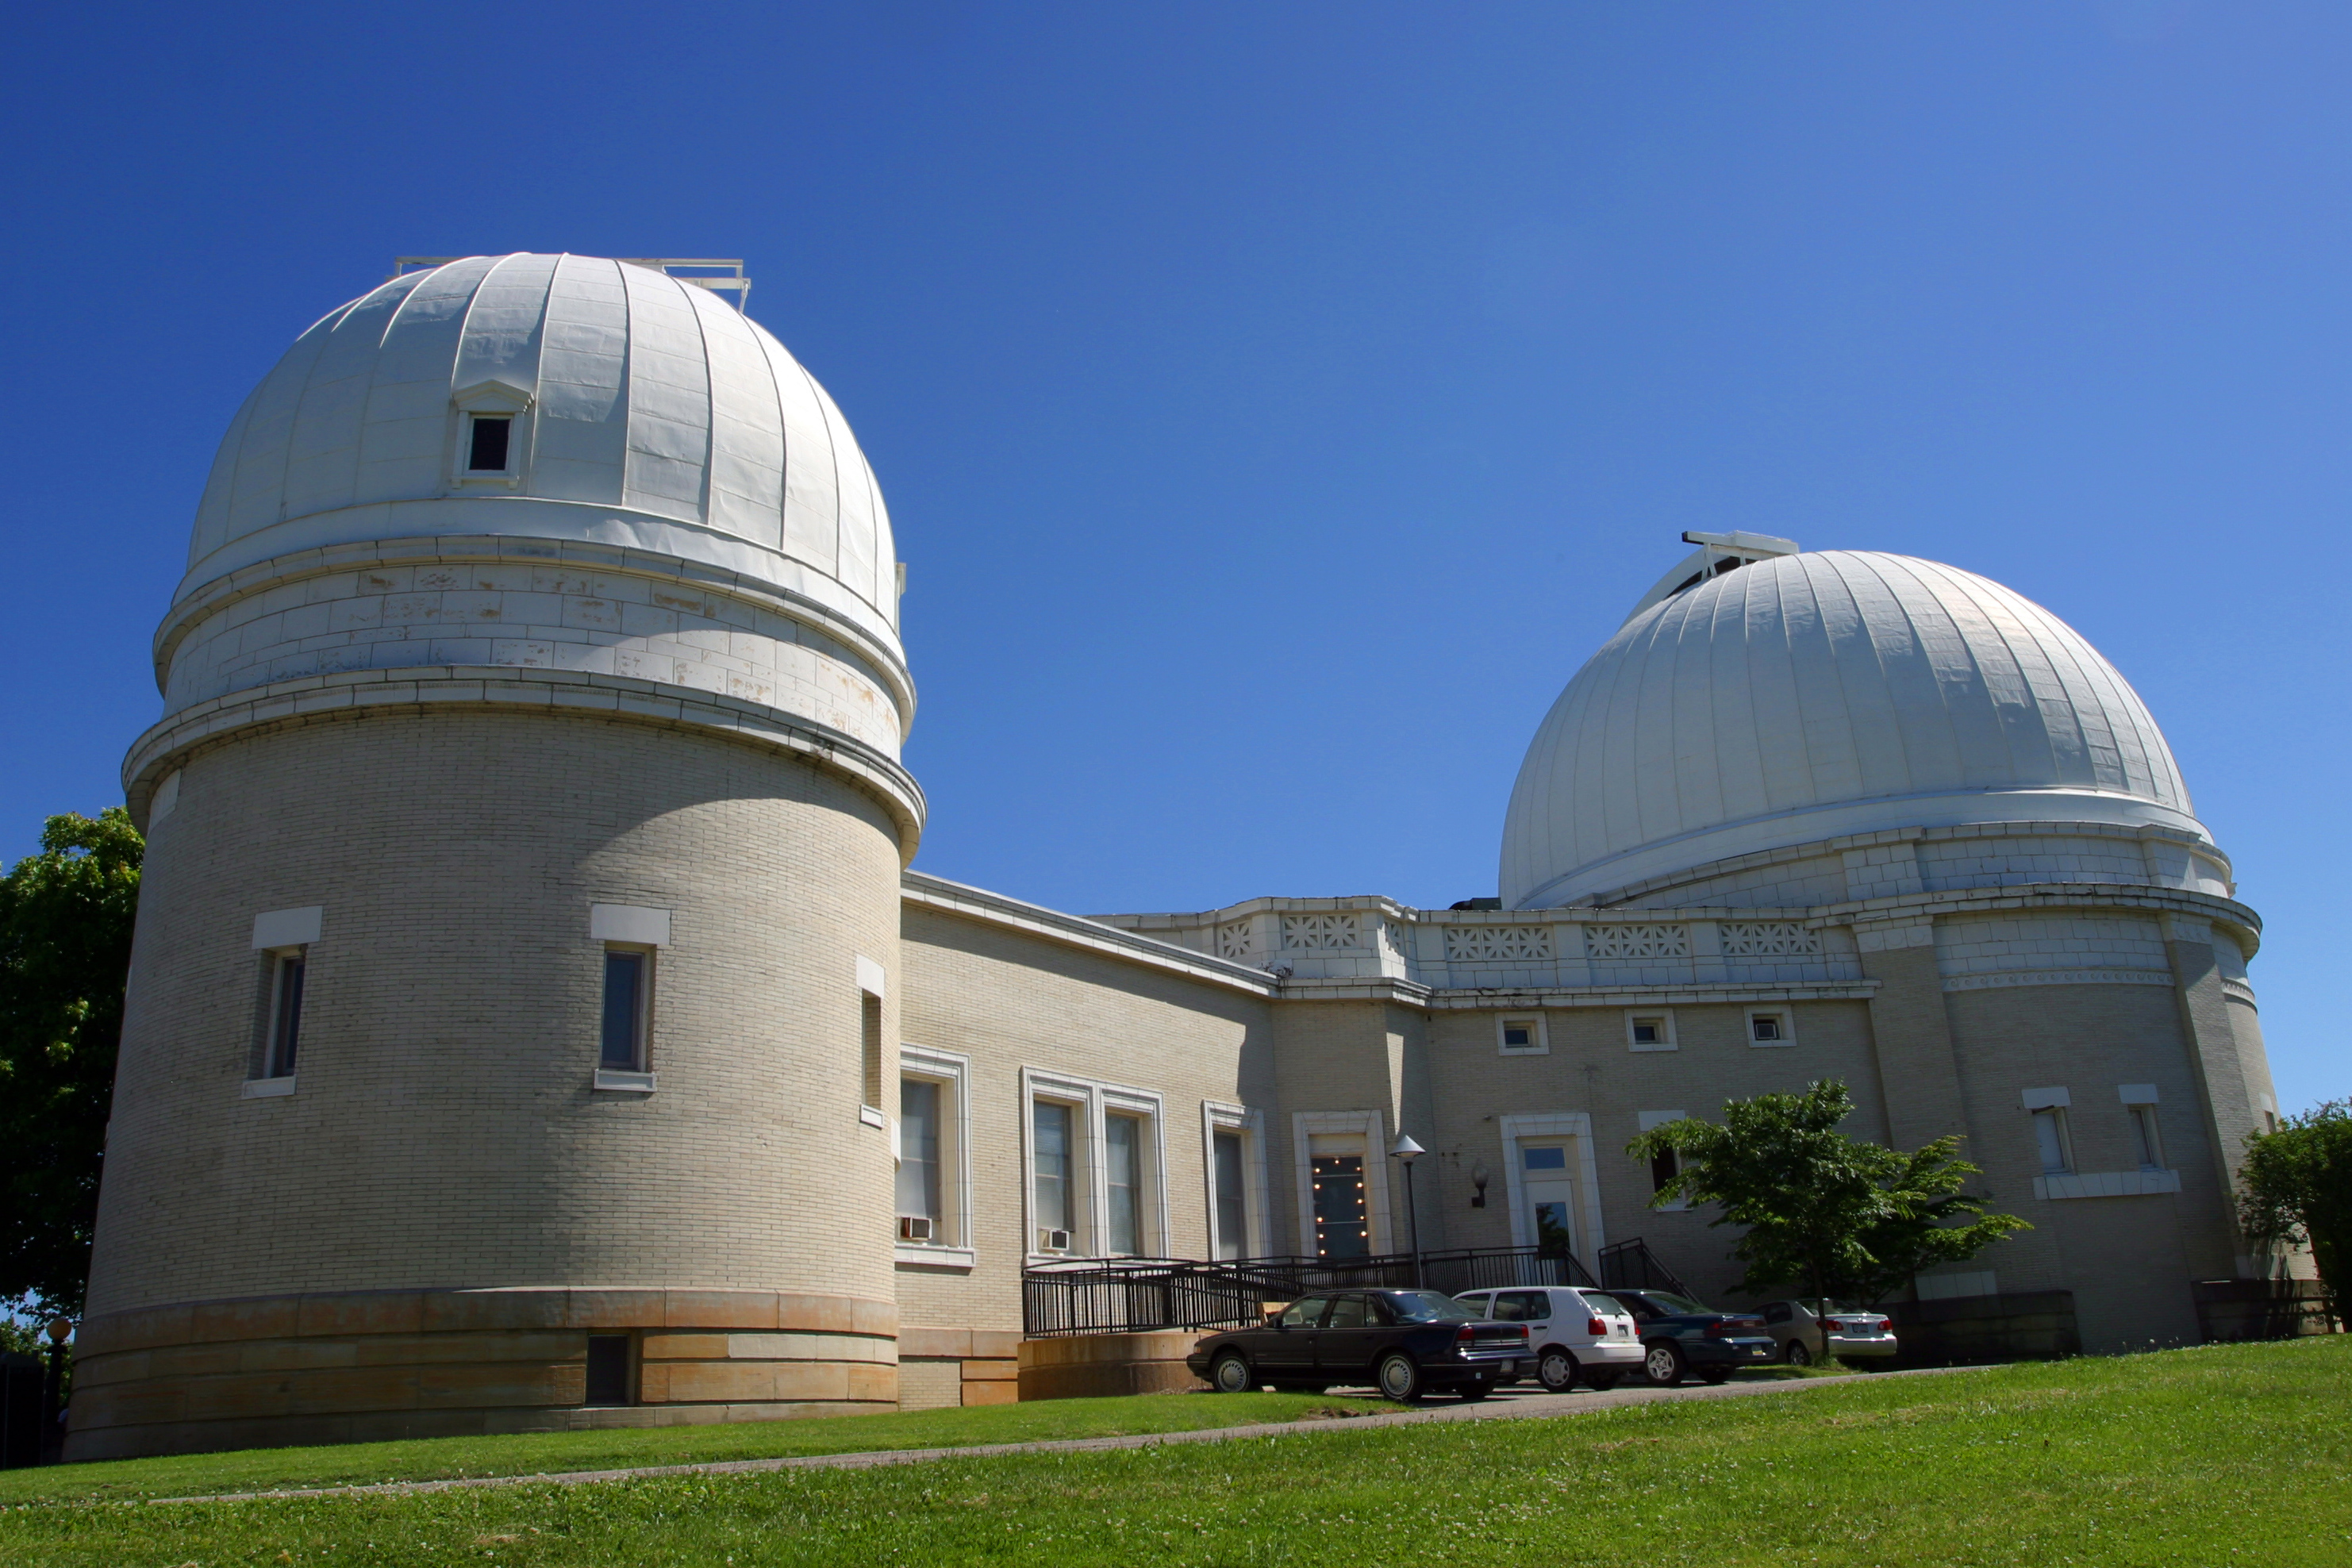
\includegraphics[totalheight=.5\textheight]{Title.jpg}
\end{center}
\begin{center}
\emph{Allegheny Observatory}
\end{center}
\end{figure}

\vfill
\begin{minipage}{0.4\textwidth}
\begin{flushleft} \large
\emph{Author:}\d\
STEPUP Team
\end{flushleft}
\end{minipage}
\begin{minipage}{0.4\textwidth}
\begin{flushright} \large
\emph{Supervisor:} \\
Professor Wood-Vasey
\end{flushright}
\end{minipage}

\end{center}
\end{titlepage}
%%%%%%%%%%%%%%%%%%%%%%%%%%%%%%%%%%%%%%%%%%%%%%%%%%%%%%%%%%%%%%%%%%%%%%%%%%%%
\tableofcontents
\chapter{Opening Checklist} 
	
Chapter 1 and 2 provide instructions on the complete observing process for STEPUP purposes. The following instructions do not require any knowledge of physics or astronomy. Therefore, anyone who can read and follow instructions can observe. If you are an experienced observer, please go to Chapter 2 for an abridged opening checklist. Please refer to Chapter 4 for troubleshooting information.

\section{Checking the Conditions}

\begin{itemize}
\item Use Pittsburgh Clear Sky Chart (http://cleardarksky.com/c/PittsburghPAkey.html) during the days before to check the possibility of observing that night. 
\item The day of, check NOAA's IR maps (http://www.goes.noaa.gov/ECIR4.html) to look at cloud cover in addition to Pittsburgh Clear Dark Sky.
\item At 7:15pm you can start checking the All Sky Camera on Allegheny Observatory's website (http://www.pitt.edu/{\textasciitilde}aobsvtry/All-Sky.html) to directly verify the cloud coverage at the observatory. Looking out the window yourself has also shown to be a good way of checking for clouds.
\end{itemize}

\section{Preliminary Setup}

\begin{itemize}
\item Log on to Ptolemy and open up the terminal
\item Create a directory for the target you are observing in the raw folder (/home/depot/STEPUP/raw) if one does not exist already. Within this newly created directory, make a directory for the data you will take that day in the format of year-month-day. So if you are observing the target HAT-P-13 on November 12, 2013, you should type {\bf mkdir /home/depot/STEPUP/raw/HAT-P-13/2013-11-12 \bf} 
\item Go into the directory you just created using the command {\bf cd /home/depot/STEPUP/raw/ \emph{target}/\emph{date})\bf} and open a blank text file named 'obsreport'. This is done by typing {\bf emacs obsreport \&} at the UNIX command prompt. You will type your observing report here. See the appendix for a sample observing report.
\item On the Lamashtu computer, open the terminal and type: {\bf vncviewer 136.142.17.99}. A prompt will ask you for a password, which is {\bf ccd}. You want to record four pieces of information in the observing report: \emph{cloud coverage, temperature, wind, and humidity}. They are located on the ClarityII window while the seeing camera is shown as a plot. 
\end{itemize}
	
\section{General Startup} 

\begin{enumerate}
\item On the Ptolemy computer, open the terminal and type: {\bf vncviewer ao-keeler.phyast.pitt.edu}. A prompt will ask you for a password, which is {\bf foo}. If the computer is not logged on, you will have to log on with the password: {\bf group1}. The username should be defaulted as \emph{group1}, but if it isn't, change the username to \emph{group1}. The username and password are the same. 
\item Open the {\bf Logitech QuickCam} on the desktop. When a window pops up, click on the first icon in that window. Use this to monitor the movement of the telescope and dome.
\item Open the {\bf Keeler Power Controller 1.1} on the desktop. You will see a series of on and off buttons. Turn the telescope on first (an automated one minute waiting period follows) followed by the rest of the controls. After you have turned on the {\bf Lens Cap Power}, click on the \emph{Open} button under {\bf Lens Cap}. View the webcam to make sure the lens cap is opening. 
\item Open the {\bf Digital Dome Works} on the desktop. Two windows should pop up: \emph{Digital DomeWorks v5.2} and \emph{RCX Control}. {\bf WARNING: KEEP THE RCX WINDOW ON LEFT SIDE OF SCREEN. IT MUST NOT MOVE TO THE RIGHT HALF OF THE SCREEN!} If the RCX window even briefly edges over to right side of screen, call Lou. 
\item Open the {\bf MaxIM DL} on the desktop. When the MaxIM window pops up, click on the {\bf Toggle CCD Control} button in the row near the top of the window. When the MaxIM CCD window opens, you should be in the \emph{Setup} tab. Click on the \emph{Connect} button followed by the \emph{Cooler On} button. 
\item Still in the MaxIM DL window, click on the {\bf Toggle Telescope Control} button in the same row near the top of the window. When the Telescope Control window opens, you should be in the \emph{Setup} tab. Click \emph{Connect} for both the telescope and focuser.
\end{enumerate}

\section{Calibration}

You should be taking calibrations each night that you observe. However, if you have time constraints (For example, if a transit starts at 9pm, but you just started setting up at 8:15pm.), you can skip this section and save it for the end of the night. 
\begin{enumerate}
\item In the Digital DomeWorks window, click on \emph{Go To} and enter 270 when it prompts you to. The dome will likely stop shy of 270 degrees, so you will need to over shoot and click \emph{STOP} a few degrees before it reaches 270. You may have to play with it a few times before the dome is positioned correctly. Use the webcam to verify the dome is moving. 
\item In the RCX Control window, turn tracking off by clicking on the green button that says \emph{Tracking} near the top. If there is a red button labeled \emph{Not Tracking}, then it is already set. Regardless, the final setting should be \emph{Not Tracking}.
\item In the RCX Control window, note the \emph{ALT} and \emph{AZ} values in the top right corner of the window. You want to set these to {\bf ALT: 10 degrees} and {\bf AZ: 180 degrees}. Within one degree is close enough. To do this, you will use the buttons in the \emph{Motion Control} box in the center of the RCX Control window. Use 'N' and 'S' buttons to adjust the ALT value larger and smaller respectively. Use the 'W' and 'E' to adjust the AZ value larger and smaller respectively. The radio buttons below labeled \emph{Guide, Center, Find, Slew} represent the magnitude of the response with \emph{Slew} being the greatest and \emph{Guide} the smallest. For example, if the ALT is at 40 deg, you will want to use \emph{Slew}, but if it is at 11 deg, you will want to use \emph{Guide}. If the direction arrows do not work, select \emph{Guide} first and try. This will wake the program up if frozen.
\item You will now create a folder to store the nights images. Click on the Start menu -{$>$} My Computer -{$>$} group 1 on 'aoserver1{$\backslash$}data'(Z:) -{$>$} STEPUPDataFiles. In this folder, create a new folder in the format of YYYY-MM-DD for the night of observation.
\item In the MaxIM CCD subwindow within the MaxIM DL window, click on the \emph{Sequence} tab. Click on \emph{Options} and select \emph{Set Destination Path...} Select the folder you just created.
\item Click on \emph{Options} again and select the \emph{Setup Sequence} choice. Enable the two boxes Flat and Bias, setting the suffix as F and B respectively. Make sure the \emph{Binning} is set to 1 and \emph{Repeat} is set to 11 for each. No other settings should be enabled at this point. {\bf IMPORTANT:} The bias images are instantaneous. This should be on default so the \emph{Exposure} cannot be changed. The flat images have exposure times of 2 seconds. Your setup should look like the screenshot below. 

\begin{figure}[!h]
\begin{center}
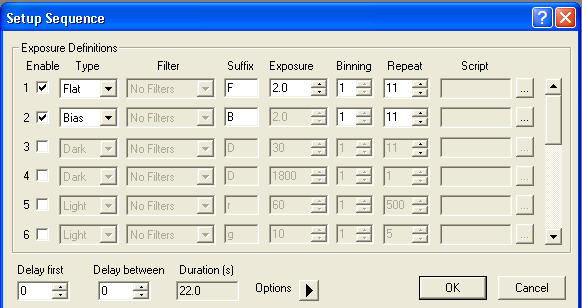
\includegraphics[totalheight=.2\textheight]{Calib.png}
\end{center}
\end{figure}

\item Still in the \emph{Sequence} tab, enter the name of the star in the \emph{Autosave Filename} box. Make sure that "1" is selected in the \emph{Start at} box. 
\item Start taking the calibration images by clicking \emph{Start}. As the images begin to download, open the folder you created. Make sure the calibration images are saving to that folder. You also want to make sure that the flat field lights are on.
\end{enumerate}

Side-note: We also take 30 minute dark calibration images, but this only needs to be done once a month and is usually not done on an observing night due to the fact that it takes over 1.5 hours. To take the 30 min darks the telescope and dome can be left where they are. In the Sequence tab instead of selecting Flat and Bias select Dark and put the exposure time at 1800 seconds (30 min). Other than that the procedure is the same.

\section{Focusing}

\begin{enumerate}
\item In Digital DomeWorks, move the dome back to 180 degrees using the \emph{Go To} setting. When it nears 180 degrees, click \emph{Home}. It should say that "Dome is Home" and "DSR closed". If not, continue to click \emph{Home} until it says "Dome is Home"
\item Still in Digital DomeWorks, click the \emph{Open} tab. This will open the dome shutters. Use the webcam to visually verify that the shutters of the dome are in fact opening. 
\item Open {\bf Starry Night College 6} on the desktop (If it asks for updates, do not update. If it asks for downloads, do not download). When the window opens click on the \emph{Telescope} tab on the left side of the screen. Then click \emph{Connect}. Minimize the \emph{Telescope} tab. Do not use these tabs again until closing.
\item In Digital DomeWorks, check the \emph{Slave to Telescope} box in the lower left corner. 
\item Open {\bf STVRemote} on the desktop. Click on the \emph{Link} tab at the top and select \emph{Establish Link (Com 3)}. Click on the \emph{Image} button once. Using the buttons under the \emph{Value} button, adjust the exposure time to 1.5 seconds. Finally, click the \emph{Monitor} button twice. 
\item In Starry Night College 6, click on the \emph{Options} tab on the top menu bar. Go to \emph{Orientation} and select \emph{Equatorial}. Go to the \emph{Edit} tab on the top menu bar and select \emph{Centre On...} Enter the target coordinates. 
\item Zoom in to the smaller rectangular box that should be labeled "Meade RCX-400.." The zoom controls are in the upper right corner of the window. Find a 6-8 magnitude star nearby that is not a binary star system by moving your cursor over the stars. Right click on the star and select \emph{slew telescope here}. You should see a red cross hair cursor move to that point. This cursor indicates where the telescope is pointing. 
\item Visually check on the webcam monitor that the telescope is pointing through the opening in the dome. Turn off flat field lights in the Keeler Power Controller 1.1.
\item In MaxIM CCD window, go to the \emph{Focus} tab. Click on the \emph{CCD} radio button. {\bf Make sure binning is set to 3 when CCD radio button is selected!} Set the exposure time between 1-5 seconds depending on quality of image. \emph{Delay} should be set at 0. Click \emph{Start Focus}. A window of the field of view will open. Click \emph{Stop}. Find the focus star in that image, right click on it and select \emph{point telescope here}.
\item Go back to Starry Night College 6.  The red cursor may or may not have shifted a bit. Right click on the focus star and select \emph{sync on 'starname'}. 
\item Open {\bf FocusMax}, which should be in the taskbar (It opened automatically when you connected the focuser). Click \emph{Focus}. Record the {\bf HFD} that FocusMax returns in the observing report. Also, under the \emph{Inspect} tab of MaxIM CCD, record both the {\bf FWHM} and {\bf HFD} values. 
\end{enumerate}

\section{Guiding}

\begin{enumerate}
\item In Starry Night College 6, re-enter the target coordinates by going to \emph{Edit} -{$>$} \emph{Centre On..} . Zoom into smaller rectangular box. Move the rectangular box around until a guide star is located in the guide star box (the smaller box above)  {\bf AND} the target star is still within the rectangular box. Ideally, we do not want the target star too far from the center. Right click on the center of the rectangular box (not the target!) and select \emph{slew telescope here}.
\item In the MaxIM CCD \emph{Focus} tab, click the \emph{Guider} radio button and set the exposure time to 3 seconds. Click \emph{Start Focus}. The guide star should show up in the image that pops up. Click \emph{Stop}. \emph{**Note: If the guide star does not show up, see Chapter 5: Troubleshooting}
\item Still in MaxIM CCD, go to the \emph{Guide} tab and select the \emph{Expose} radio button. Make sure the exposure time is set to 3 seconds. Click \emph{Start}. An image with the guide star should pop up. Click on the guide star in the image. Back in the \emph{Guide} tab, select the \emph{Track} radio button and click \emph{Start}. A very small image window with the guide star should show up. Monitor this window occasionally to ensure the guide star is still present and appears in focus. 
\end{enumerate}

\section{Sequencing}

\begin{enumerate}
\item In MaxIM CCD \emph{Sequence} tab, click on \emph{Options} -{$>$} \emph{Setup Sequence}. Uncheck the calibration images. Check a box where \emph{Light} is selected. Select the appropriate filter and suffix (r' for exoplanets). Select an exposure time depending on the magnitude of the target star, normally between 30-120 seconds. Click \emph{Ok}.
\item Back in the \emph{Sequence} tab, make sure the image starts at 1 and the target star name is in the \emph{Autosave Filename} box. Click \emph{Start}.
\item After the image downloads, click on the cross hair button near the top of the MaxIM DL screen. A circular aperature now becomes your cursor and a small window with information about the pixel counts should pop up. Move the circular cursor over the target star. If the counts are between 20,000-50,000, then you are set. Record the {\bf FWHM, Maximum, Minimum, Bgd Avg} in the observing report. You will record this information every 30 minutes. If the counts are below 20,000, you will want to increase the exposure time. If the counts are above 50,000, you will want to decrease the exposure time. 
\item If the maximum hits 65,535 this means the ccd has been maxed out. If the target star hits 65,535 in an image than we \emph{cannot} use that image in our data analysis. 
\item Try to keep the exposure time below 200s so we get a decent number of images of the the transit. If you observing a star dimmer than magnitude 11.5, this may mean that the maximum counts dip to around 10,000. That's okay, as long at its remains above 7,500 the data should be analyzable, just slightly noiser. 
\end{enumerate}

\chapter{Abridged Opening Checklist}

\begin{enumerate}
\item Open all controls in the {\bf Keeler Power Controller 1.1}.
\item Open Logitech webcam. 
\item Open {\bf Digital Dome Works}. {\bf Remember to keep RCX window on left side of the screen!!!}
\item Open {\bf MaxIM DL}. Open {\bf Toggle CCD Control} and click both \emph{Connect} and \emph{Cooler On}. Open {\bf Toggle Telescope Control} and connect both focuser and telescope.
\item Open {\bf STVRemote}. Under the \emph{Link} tab, click on \emph{Establish Link (Com 3)}. Click \emph{Image} button once. Set exposure time to 1.5 seconds. Click \emph{Monitor} twice. 
\item Create folder for the night in STEPUPDataFiles under the Z drive.
\item Set destination path to that folder in MaxIM CCD.
\item {\bf Calibrations}
\begin{enumerate}
\item Move telescope to {\bf ALT: 10 deg} and {\bf AZ: 180 deg} in the RCX window.
\item Move dome to 270 deg. 
\item Ensure flat field lights are on.
\item In MaxIM, setup the sequence with 11 images each of the flats and biases. Flats should be 2 seconds and biases are instantaneous. The suffixes are F and B. 
\item Make sure image starts at 1 and the filename is the name of the star you are observing. 
\item Click \emph{Start}.
\end{enumerate}
\item Move dome back to 180. Click \emph{Home} and make sure DDW says it is home. Open the shutters. Click \emph{Slave to Telescope}.
\item Open {\bf Starry Night College 6}. 
\begin{enumerate}
\item Connect the telescope. 
\item Set orientation to \emph{Equatorial} .
\item Center onto the target coordinates. Right click on the field of view and select \emph{Point Telescope Here}.
\item Select a star between the magnitudes 6-8 nearby. 
\end{enumerate}
\item Go to MaxIM DL. In the \emph{Focus} tab, select CCD radio button and start 1-5 second focus. {\bf Make sure binning is set to 3 when CCD radio button is selected!} Right click on target star and select \emph{Point telescope here}.
\item Back in Starry Night, right click on focus star and select \emph{sync to 'starname'}.
\item {\bf Turn off flat field lights!}
\item Go to FocusMax and click \emph{Focus}. Record the {\bf HFD} and {\bf FWHM} info from both FocusMax and MaxIM.
\item Re-enter coordinates in Starry Night. Put a guide star in the guide star box. Right click on center of field of view and select \emph{Point telescope here}.
\item In MaxIM Focus tab, select the \emph{Guide} radio button and click \emph{Start Focus}. Make sure the guide star is there.
\item In MaxIM Guide tab, select the \emph{Expose} radio button and click \emph{Start}. Click on the guide star in the image that pops up. Back in the Guide tab, select the \emph{Track} radio button and click \emph{Start}. 
\item In MaxIM Sequence tab, setup the sequence so the light images are being taken. Make sure image starts at 1 and the \emph{Autosave Filename} is filled in with target star name. 
\end{enumerate}

\chapter{Closing Checklist}

\begin{enumerate}
\item Under the \emph{Setup} tab in the MaxIM CCD window, press the \emph{Warm Up} button. Wait about 1 minute. Click on \emph{Cooler Off}. Click on \emph{Disconnect}.
\item In the MaxIM Telescope Control window, click \emph{Disconnect} for both the telescpe and focuser.
\item Exit MaxIM DL completely.
\item In the Starry Night College 6 program, open the \emph{Telescope} tab on the left. Disconnect the telescope. Exit Starry Night College 6.
\item In the RCX Contrl window, click on the \emph{Park} button.
\item In Digital DomeWorks, turn the dome to 180 degrees. When it stops, click \emph{Home} and make sure the message "Dome is Home" is there. Click \emph{Close} and make sure the message "DSR is CLOSED" is there. Visually check the webcam screen to ensure dome is in fact closed (If it's dark, turn on flat field lights).
\item In STVRemote, click \emph{Interrupt} and close the program.
\item In the Keeler Power Controller 1.1, click \emph{Close} under the lens cap. Make sure lens cap closes in the webcam view.
\item Close the Logitech webcam.
\item Close Digital Dome Works.
\item Turn off all the power switches in the Keeler Power Controller 1.1 starting from \emph{Lens Cap Power} up to \emph{Telescope}.
\item Log off the computer.
\end{enumerate}

\chapter{Troubleshooting}

\section{WinTV}

WinTV shows the image that the finder camera sees. The image is not as clear, but you should be able to see a few bright stars in WinTV. Match these stars with those in the images that you take. If the the stars do not match up, the telescope is not pointed at where Starry Night says it is pointed.
\begin{itemize}
\item Click \emph{start -{$>$} Remote Desktop Connection}. Log onto 136.142.17.105. The password is {\bf blah}
\end{itemize}

\section{No stars in Image}

\begin{itemize}
\item Did you turn off the flat field lights? Use webcam to check.
\item Are the shutters of the dome opened? Use webcam to check. If DDW says it is open, but the webcam shows it is not, move the dome back to 180. Click \emph{Home}. Click \emph{Close}. Click \emph{Reset}. Click \emph{Open}. If the dome still does not open, call Lou.
\item What does the All Sky Camera show? Are there thick clouds?
\item Check the sequence setup. Make sure we are taking images in R or r'.
\item Did the dome get stuck? If so, \emph{See Dome}.
\item Is the dome still slaved to the telescope? If not, recheck that box in DDW.
\end{itemize}

\section{Wrong star field}

\begin{itemize}
\item \emph{See WinTV}
\item Did daylight savings recently happen? If so, call Lou.
\item Go to Edit -{$>$} Centre On. Re-enter the target coordinates. Make sure the coordinates are correct before centering.
\end{itemize}

\section{Dome}
\begin{itemize}
\item If DDW shows the shutters are opened, but it is not, close the shutters in DDW. Click \emph{reset}. Reopen the shutters. If it does not work, call Lou.
\item If the dome is stuck, unslave the telescope. Move the dome in the opposite direction it was going by at least 90 degrees. Reslave the telescope. If the dome still gets stuck, more the dome in the opposite direction by at least 181 degrees. Then reslave the telescope. The dome should now reach where the telescope is from the other direction. \emph{Note: In the winter, the dome sometimes gets stuck in the 300-360 degree range.}
\end{itemize}

\section{Not focusing}
\begin{itemize}
\item If you are having trouble focusing, try focusing on a magnitude 6ish star that is dirctly overhead (sidereal time equals star's RA) and a declination of 40 degrees.
\item If you are unsure if the telescope is working (i.e. it is so out of focus you can't see anything) try pointing it at a really bright star such as Vega, Capella, Polaris or even Sirius. While you might be able to see these stars as bright blobs taking up half of the viewing window you won't be able to focus on them since they are so bright. However, they do serve as a good indicator that the telescope is working and pointing where you tell it to go.
\end{itemize}


\chapter{Appendix}

\section{Sample Observing Report}

\begin{verbatim}
Observers: Daniel, Megan, Lydia, Zoe

Conditions
Cloud Cover: Clear
Wind: 4.1 mph
Humidity: 38%
Temperature: 35.6 F

Target: WASP-65  mag: 11.9
RA: 08:53:17.83     Dec: 08:31:22.8

4:45pm - Checked to make sure dome and telescope were functioning properly

5:05pm - started taking dark calibrations

7:30pm - started taking flat and bias calibrations

8:13pm - focused telescope

MaxIM: FWHM: 2.91      HFD: 4.63

8:35pm - started guiding 

Guide star:TYC811-2091-1    mag: 10.12
RA: 8:53:50.3        Dec: 8:43:01

8:40pm - Started sequenc08

Filter: r'     Exp Time:120sec

    001r      FWHM = 5.3        
          Star(max) = 16873    
              
8:47pm 

     003r      FWHM = 3.957        Star(min) = 4565
          Star(max) =21438    Bkgr(avg) = 4688

For image 4 we lost the guider and the image was completely blank. It looked
like a dark calibration image. Asof 9:10 it seems to have recovered and all of
our images look normal
              
9:30pm 

     014r      FWHM = 6.364        Star(min) = 3810
          Star(max) = 21334    Bkgr(avg) = 3906
           
10:00pm

     021r      FWHM = 8.138        Star(min) = 4327
          Star(max) = 12939    Bkgr(avg) = 4429
              
10:19pm - refocused, but didn't seem to get any better. Images look okay though.

     024r      FWHM = 9.716        Star(min) = 4114
          Star(max) = 11707    Bkgr(avg) = 4229
              
11:00pm - FWHM over 10 now, tried to refocus again. Refocused 3 times, 
FWHM of focus star was 7. Wind reading from enviroment computer has
been above 8 mph. Might be causing bad seeing?

    036r      FWHM = 10.499     Star(min) = 4034
          Star(max) = 9225    Bkgr(avg) = 4118
              
11:30pm 

     041r      FWHM = 10.936        Star(min) = 4009.000
          Star(max) = 8781.000    Bkgr(avg) = 4096.425
         
12:01pm 

     049r      FWHM = 10.320        Star(min) = 3891.000
          Star(max) = 9865.000    Bkgr(avg) = 3951.282
        
12:34pm 

     058r      FWHM = 11.374        Star(min) = 3850.000
          Star(max) = 8807.000    Bkgr(avg) = 3901.535

12:45pm - Shut down
\end{verbatim}



\end{document}
